\chapter{Baggrund}

Det primære produkt Responsum K/S leverer til sine kunder er receptionister. Alle virksomheder har behov for at få  besvaret telefoner i forskellige sammenhænge, og alle virksomheder har som problem at denne funktion ofte er særdeles besværlig at have med at gøre. 

For store og mellemstore virksomheder er receptionen ofte en omkostningstung affære, som ingen rigtig har lyst til at beskæftige sig med. Der er svære udfordringer hvad angår både teknik og personale. Man har ofte åbent længere end hvad en almindelig arbejdsuge kan dække, og der skal tages hensyn til fravær. Det bliver meget hurtigt meget dyrt. Ydermere er der kun ringe prestige i at få en reception til at fungere godt, så i en større organisation betragter medarbejdere dette felt som en blind vej for karrieren. Disse forhold gør at mange organisationer ender med at outsource receptionen.

For mindre virksomheder er det et helt basalt praktisk problem at få svaret telefonen når gamle og nye kunder ringer ind. Man har ikke omsætning nok til overhovedet at overveje at have en dedikeret person til at svare kald og de få medarbejdere der er i virksomheden er optaget af at udføre de opgaver virksomheden lever af. Forretninger med få medarbejdere må ofte se kald blive mistet eller sendt til en telefonsvarer på grund af tidspres. Ingen af delene er acceptabelt for en moderne forretning.
Responsum K/S sørger for antagelse, uddannelse og fastholdelse af personale til at varetage alle opgaver relateret til håndtering af indgående kald i en organisation. De sørger for at fordele kald og beskeder indad i organisationen, og de sørger for kontinuerligt at uddanne deres receptionister så de er klædt på til at håndtere en meget bred vifte af brancher og kaldtyper.

Responsum K/S benytter sig af et relativt kompliceret teknisk system til at levere deres service. For at kunne svare kald skal de bruge telefonsystemer der kan håndtere meget store mængder telefonnumre og tilsvarende store mængder teletrafik. Deres telefonanlæg har fuld understøttelse af ting som IVR menuer, rutning af kald baseret på tid og opkalder, optagelse af samtaler, køer, automatisk eskalering af kald, statistisk/faktura værktøjer og en masse administrative værktøjer til at styre alt fra simple databaser over kontaktpersoner til dannelse og vedligeholdelse af komplicerede kaldplaner. Deres receptionister skal desuden have rimelig dyb viden tilgængelig om de virksomheder og personer de svarer kald for. Det kræver systemer hvor data hurtigt kan knyttes til kald og herefter gøres tilgængelige for receptionisterne på en overskuelig og funktionel måde.

Teknisk benytter Responsum K/S sig af et system der er udviklet i slutningen af 1990’erne, og som helt grundlæggende består af en masse sorte bokse der ikke længere udvikles på. Fra PBX’er til den PC klient receptionisterne arbejder med er der tale om lukkede systemer, som kun meget svagt kan integrere med andre systemer. Som følge heraf har Responsum K/S dagligt udfordringer hvad angår skalering og vækst, integration med moderne systemer og en hæmmende rigiditet der kommer af at leve med et stykke software hvor udvidelse og tilpasning ikke er tænkt ind fra starten.
Efter i flere år forgæves at have søgt efter noget bedre, tog Responsum K/S i november 2011 initiativ til at starte på udviklingen af et nyt telefonanlæg. Det skulle være open source, GPL licenseret og udviklerne skulle eje den forretning hvor produktet blev skabt. AdaHeads K/S blev født.

\pagebreak

\section{AdaHeads produkt}
AdaHeads' produkt bestod af systemerne der kan ses på firgur~\ref{fig:adaheadssystembefore} inden projektet gik igang. Der vil være en gennemgang i kapitel~\ref{sec:adminSystemoversigt} af hvilke nye dele der blev tilføjet.
\begin{figure}[ht!]
\centering
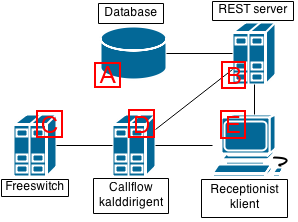
\includegraphics[scale=0.5]{images/system_before_admin.png}
\caption{En oversigt over Adaheads system.}
\label{fig:adaheadssystembefore}
\end{figure}
\begin{enumerate}
	\item[A.]{Relationel database}
	\item[B.]{REST intefaces, fordelt på flere HTTP servere}
	\item[C.]{Freeswitch PBX til håndtering af opkald} 
	\item[D.]{CallFlow kald dirigenten håndterer kaldrelateret kommunikation mellem Freeswitch og resten af systemet}
	\item[E.]{Browser baseret klient til receptionister}
\end{enumerate}
